\section{Abstract-""Syntax-""Tree (AST)}

Der Abstract-""Syntax-""Tree (AST) ist eine zentrale Datenstruktur im Programm, da jede Komponente mit ihr umgehen muss. Ableitungen und Assoziationen spiegeln direkt die Grammatik der WHILE-""Sprache wider. Da der AST von mehreren Komponenten mit unterschiedlichem Verhalten benutzt wird, bietet sich hier das "`Besucher"'-""Entwurfsmuster (siehe Kapitel \ref{astvisitor_sec}) an.

\subsection{"`Besucher"'-""Entwurfsmuster}
\label{astvisitor_sec}
Das "`Besucher"'-""Entwurfsmuster lagert die Operationen in externe Klassen (bspw. des Interpreters) aus. Somit lassen sich verschiedene, an den jeweiligen Verwendungszweck angepasste Operationen auf demselben AST ausführen. Jede Klasse erbt direkt oder indirekt durch die Ableitung der Klasse ASTNode die Methode \texttt{accept()}. Dadurch lässt sich jede Klasse im Baum durch einen \type{AST"-Node"-Visitor} besuchen.
Ein geparstes Programm liegt durch die Assoziationen als Baum vor. Dieser lässt sich mithilfe von \texttt{accept()} traversieren. Jeder Knoten des Baums kann so erreicht werden und somit ist eine vollständige Abarbeitung des Programms gewährleistet. Der jeweilige Verwendungszweck ergibt sich durch die Benutzung verschiedener \type{AST"-Node"-Visitor}-""Instanzen in der entsprechenden Komponente. 

\subsection{Klassenentwurf}
\subsubsection{abstract class ASTNode}
\label{astnode_class}
Grundsätzlich sind alle Klassen Ableitungen der Klasse \type{ASTNode} (siehe Abbildung~\ref{ast_diag}). Hierdurch wird sicher gestellt, dass jede Klasse mittels der Methode \texttt{accept()} von einem \type{AST"-Node"-Visitor} besucht werden kann. Zusätzlich bietet diese Klasse Methoden, um Rückschlüsse~(Position, Zeilennummer) auf den ursprünglichen Programmcode zu ziehen.

\subsubsection{class Program}
Ein Objekt der Klasse \type{Program} stellt den Wurzelknoten eines geparsten Programms dar. Solch ein Program kann mehrere Funktionsdeklarationen~(siehe Kapitel~\ref{astfunctiondecl_class}) und maximal einen Block~(siehe Kapitel~\ref{astblock_class}), welcher als Main-Block des Programms bezeichnet wird, enthalten. Des Weiteren kann ein Program eine Liste an Axiomen~(siehe Abbildung~\ref{ast_diag}) enthalten, welche allgemeingültige Aussagen unabhängig vom Programm festsetzen.

\subsubsection{class FunctionDeclaration}
\label{astfunctiondecl_class}
In der Klasse \type{FunctionDeclaration} werden zu der jeweiligen Funktion die Signatur~(Name, Parameter, Rückgabetyp), der Funktionskörper-""\type{Block}~(siehe Kapitel~\ref{astblock_class}) und wahlweise angegebene Vor- und Nachbedingungen~(siehe Abbildung \ref{ast_diag}) gespeichert.

\subsubsection{class Block}
\label{astblock_class}
Ein \type{Block} beinhaltet eine beliebige Anzahl an \type{Statement}s~(siehe Kapitel~\ref{aststatement_class}).

\subsubsection{abstract class Statement}
\label{aststatement_class}
Diese Klasse dient dazu, von den einzelnen \type{Statement}s~(bspw. \type{Return"-Statement}, \type{Assignment}, \type{Variable"-Declaration}, siehe auch Abbildung~\ref{ast_diag}) zu abstrahieren.

\subsubsection{abstract class Expression}
\label{astexpr_class}
Ein Ausdruck spezialisiert sich in verschiedenen Klassen wie \type{Quantified"-Expression}, \type{Literal}, und \type{Binary"-Expression}~(siehe auch Abbildung~\ref{ast_diag}).

\begin{landscape}
\begin{figure}%
    \vspace{-2cm}%
    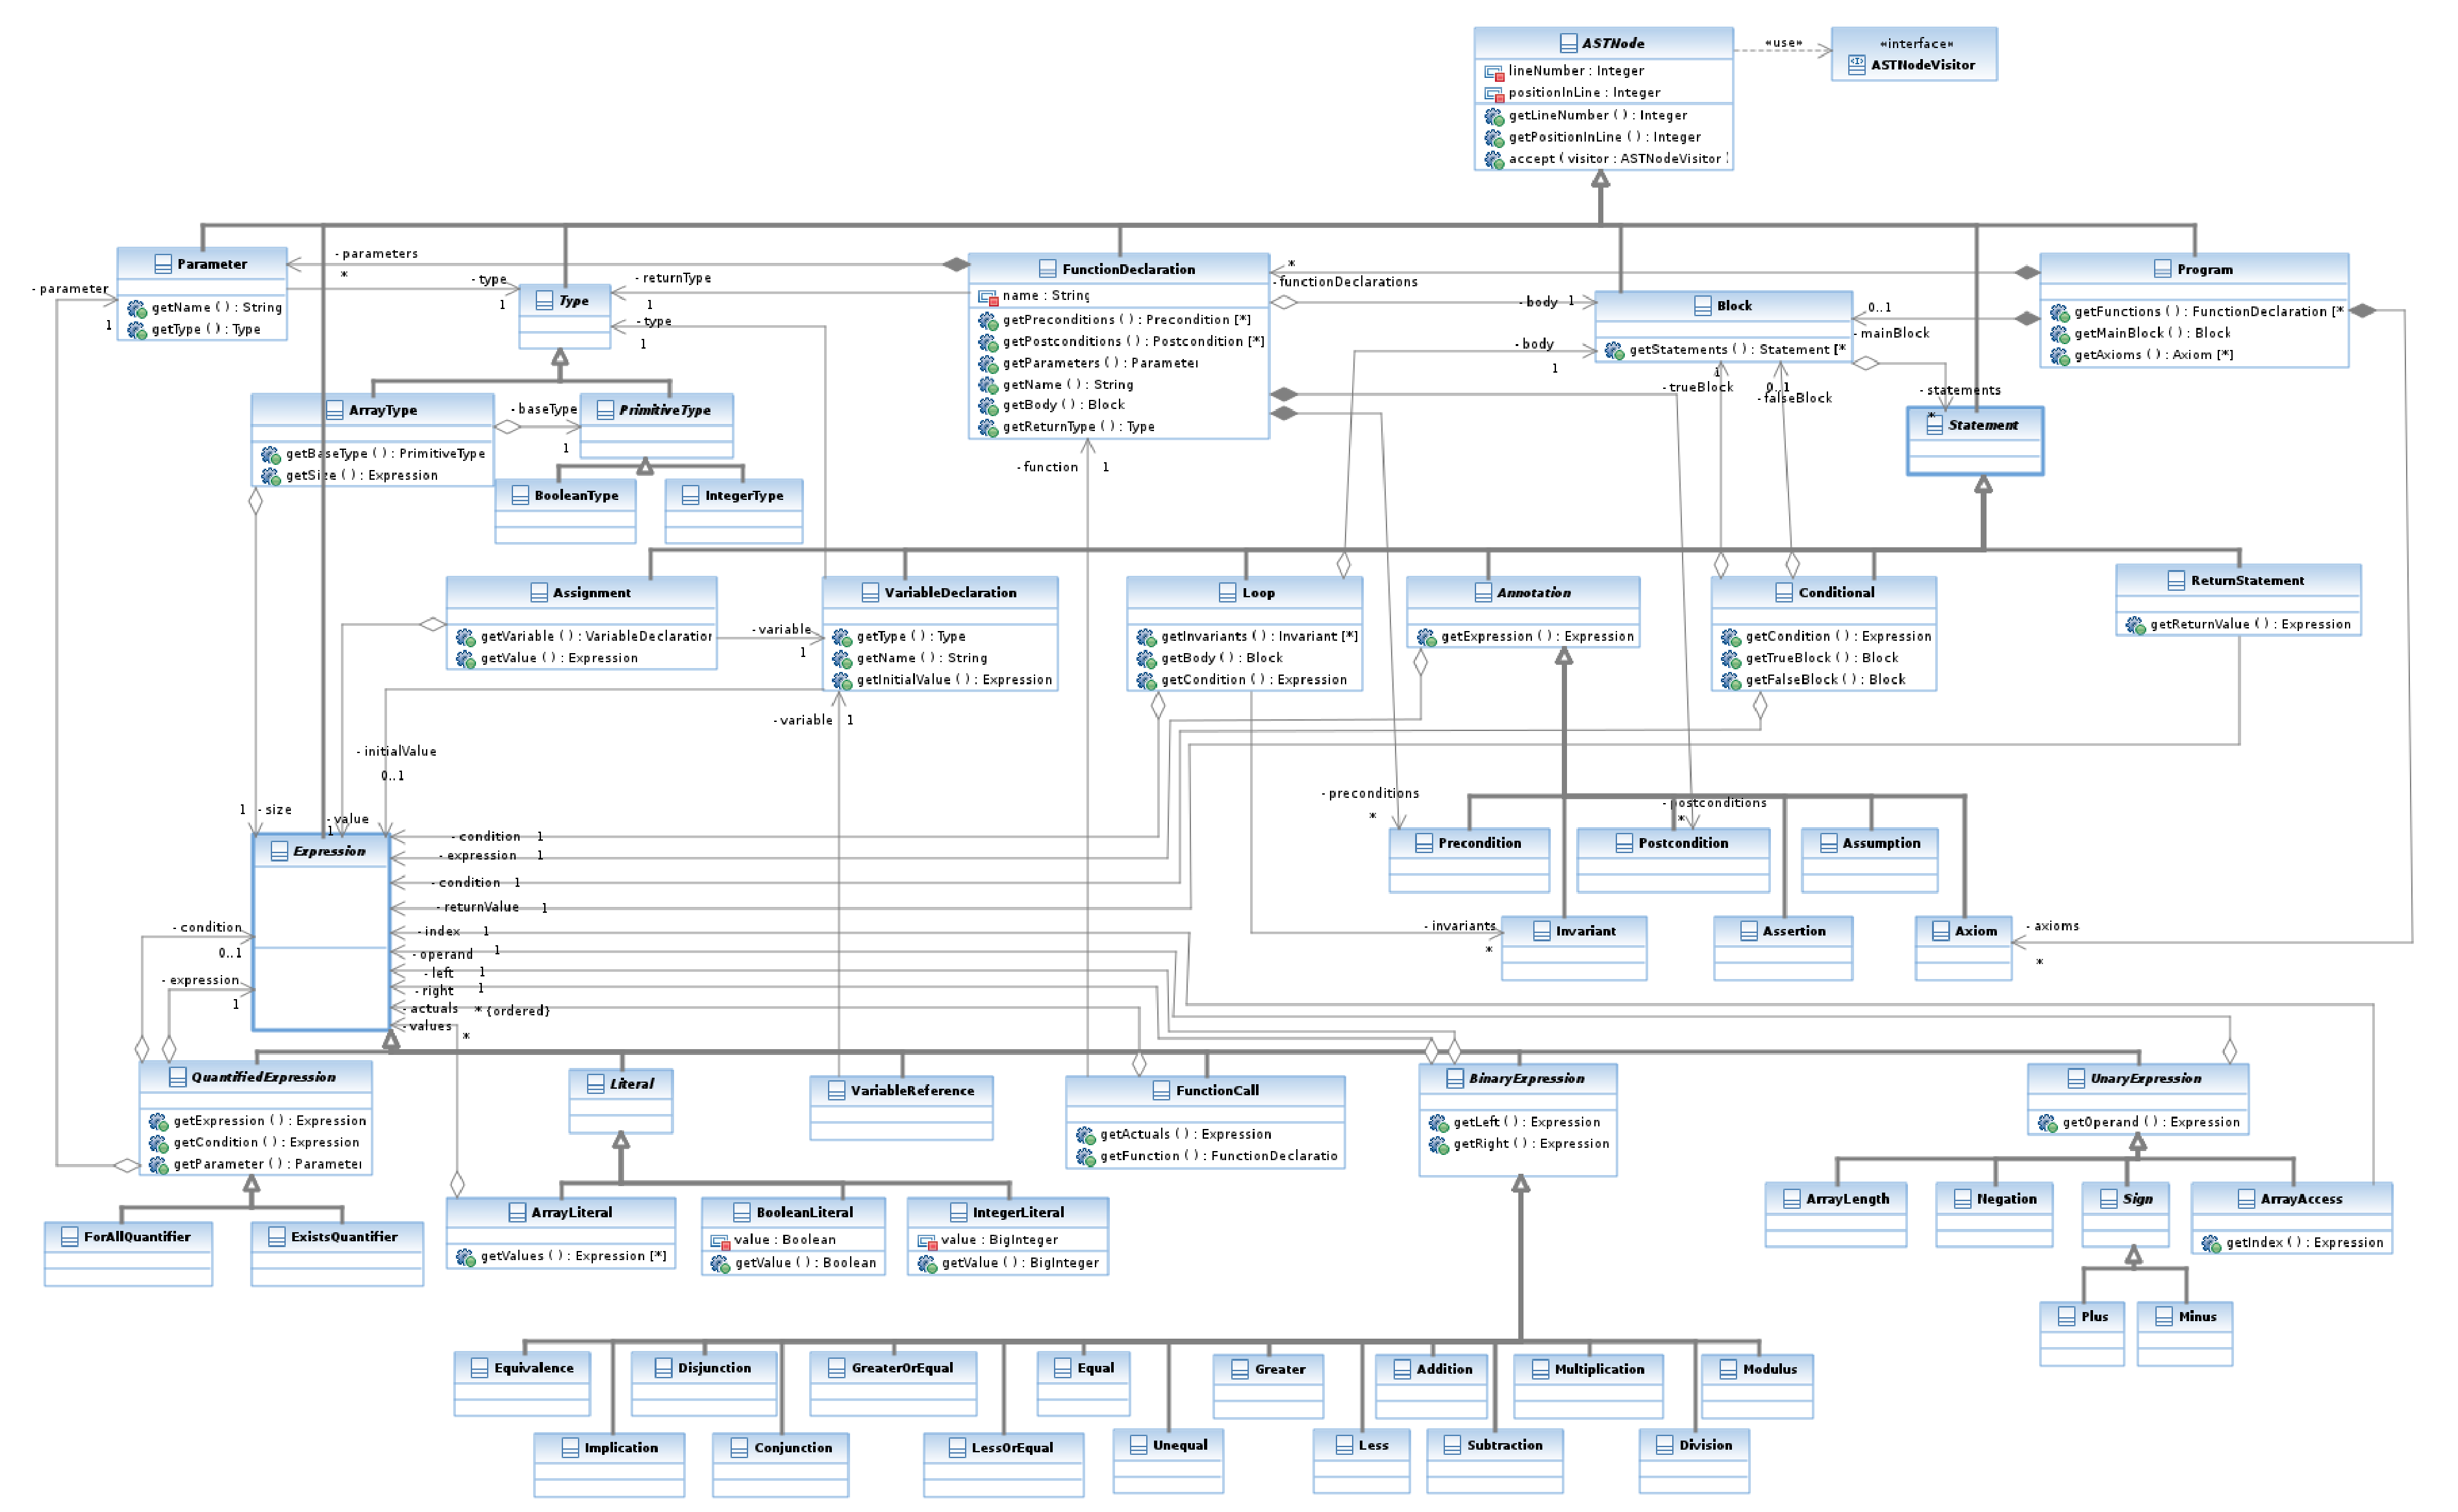
\includegraphics[height=\textheight]{diagrams/ast_component.pdf}

    \caption{Klassendiagramm des Abstract-""Syntax-""Trees mit den
    \type{Program}-""Bestandteilen \type{Statement} und
    \type{Expression} sowie der "`Besucher"'-""Klasse
    \type{AST"-Node"-Visitor}}

    \label{ast_diag}
\end{figure}%
\end{landscape}
